\documentclass[border=6pt]{standalone}
\usepackage{tikz}
\usetikzlibrary{arrows.meta,positioning,calc}
\begin{document}
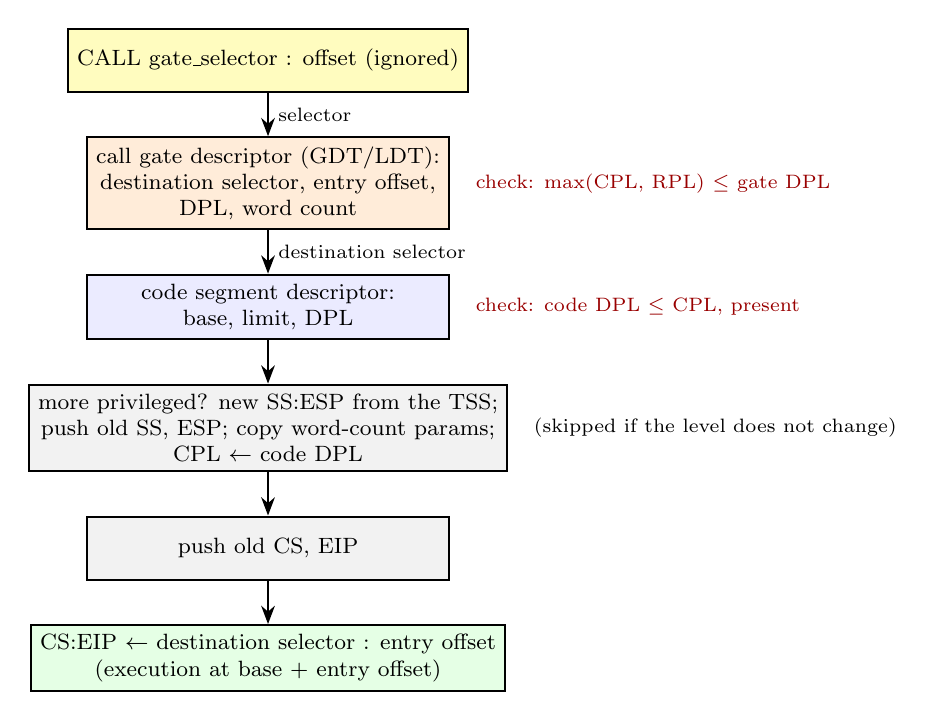
\begin{tikzpicture}[>=Stealth,font=\small,node distance=0.55cm,
 b/.style={draw,thick,align=center,font=\footnotesize,minimum height=0.8cm,minimum width=4.6cm},
 c/.style={font=\scriptsize,align=left,anchor=west}]
\node[b,fill=yellow!25] (ins) {CALL gate\_selector : offset (ignored)};
\node[b,fill=orange!15,below=of ins] (gate) {call gate descriptor (GDT/LDT):\\destination selector, entry offset,\\DPL, word count};
\node[b,fill=blue!8,below=of gate] (code) {code segment descriptor:\\base, limit, DPL};
\node[b,fill=gray!10,below=of code] (stk) {more privileged? new SS:ESP from the TSS;\\push old SS, ESP; copy word-count params;\\CPL $\leftarrow$ code DPL};
\node[b,fill=gray!10,below=of stk] (ret) {push old CS, EIP};
\node[b,fill=green!10,below=of ret] (go) {CS:EIP $\leftarrow$ destination selector : entry offset\\(execution at base + entry offset)};
\draw[->,thick] (ins) -- (gate) node[midway,right,font=\scriptsize]{selector};
\draw[->,thick] (gate) -- (code) node[midway,right,font=\scriptsize]{destination selector};
\draw[->,thick] (code) -- (stk);
\draw[->,thick] (stk) -- (ret);
\draw[->,thick] (ret) -- (go);
\node[c,red!60!black] at ($(gate.east)+(0.2,0)$) {check: max(CPL, RPL) $\le$ gate DPL};
\node[c,red!60!black] at ($(code.east)+(0.2,0)$) {check: code DPL $\le$ CPL, present};
\node[c] at ($(stk.east)+(0.2,0)$) {(skipped if the level does not change)};
\end{tikzpicture}
\end{document}
